
%使用XeLaTeX编译
%版权所有,翻版必究
%本文件由程序自动生成,任何修改将被覆盖
%2019 年 01 月 23 日




\FloatBarrier
\section{
使用C{\sourcefonttwo{}+}{\sourcefonttwo{}+}扩展Qt Quick
}\label{s100710}


读者可能认为使用Qt Quick只需要Qml足以,但不久读者就会失望。
即使退一步,希望Qt Quick可以满足绝大多数需求,这也是难以达成。

Qt Quick不是一种全面代替Qt C{\sourcefonttwo{}+}{\sourcefonttwo{}+}无所不包的解决方案。
Qt Quick只是导出Qt C{\sourcefonttwo{}+}{\sourcefonttwo{}+}的一套接口规范。

当读者面对一个具体的问题,在Qt Quick中无法找到现成的组件或者无法通过
简单修改现有Qt Quick组件达成目的时。使用Qt C{\sourcefonttwo{}+}{\sourcefonttwo{}+}自定义组件就势在必行。

\begin{itemize}

\item 如果所需的组件不需要几何逻辑,
比如实现一个本地文件监视器,那么只继承自QObject即可;

\item 如果所需的组件需要几何逻辑但无需渲染,
比如实现一个鼠标监视器,那么只需要继承自QQuickItem;

\item 如果所需的组件需要渲染,
那么需要继承自QQuickItem,并在构造函数中设置
QQuickItem::ItemHasContents标志位;

\item 如果希望使用QPainter实现渲染,
那么需要继承自QQuickPaintedItem是一个好的选择;

\item 如果仅需要一个简易的OpenGL离屏渲染环境,
那么继承自QQuickFramebufferObject是一个好的选择;

\end{itemize}

如\figurename\ \ref{p000010}
,列出了C{\sourcefonttwo{}+}{\sourcefonttwo{}+}导出Qt Quick基类继承关系图。

%begin图片
\begin{figure}[htb] %浮动体 here and top ...
%there must use marginnote ...
\marginnote{\setlength\fboxsep{2pt}\fbox{\footnotesize{\kaishu\figurename\,}\footnotesize{\ref{p000010}}}}\centering %中心对齐
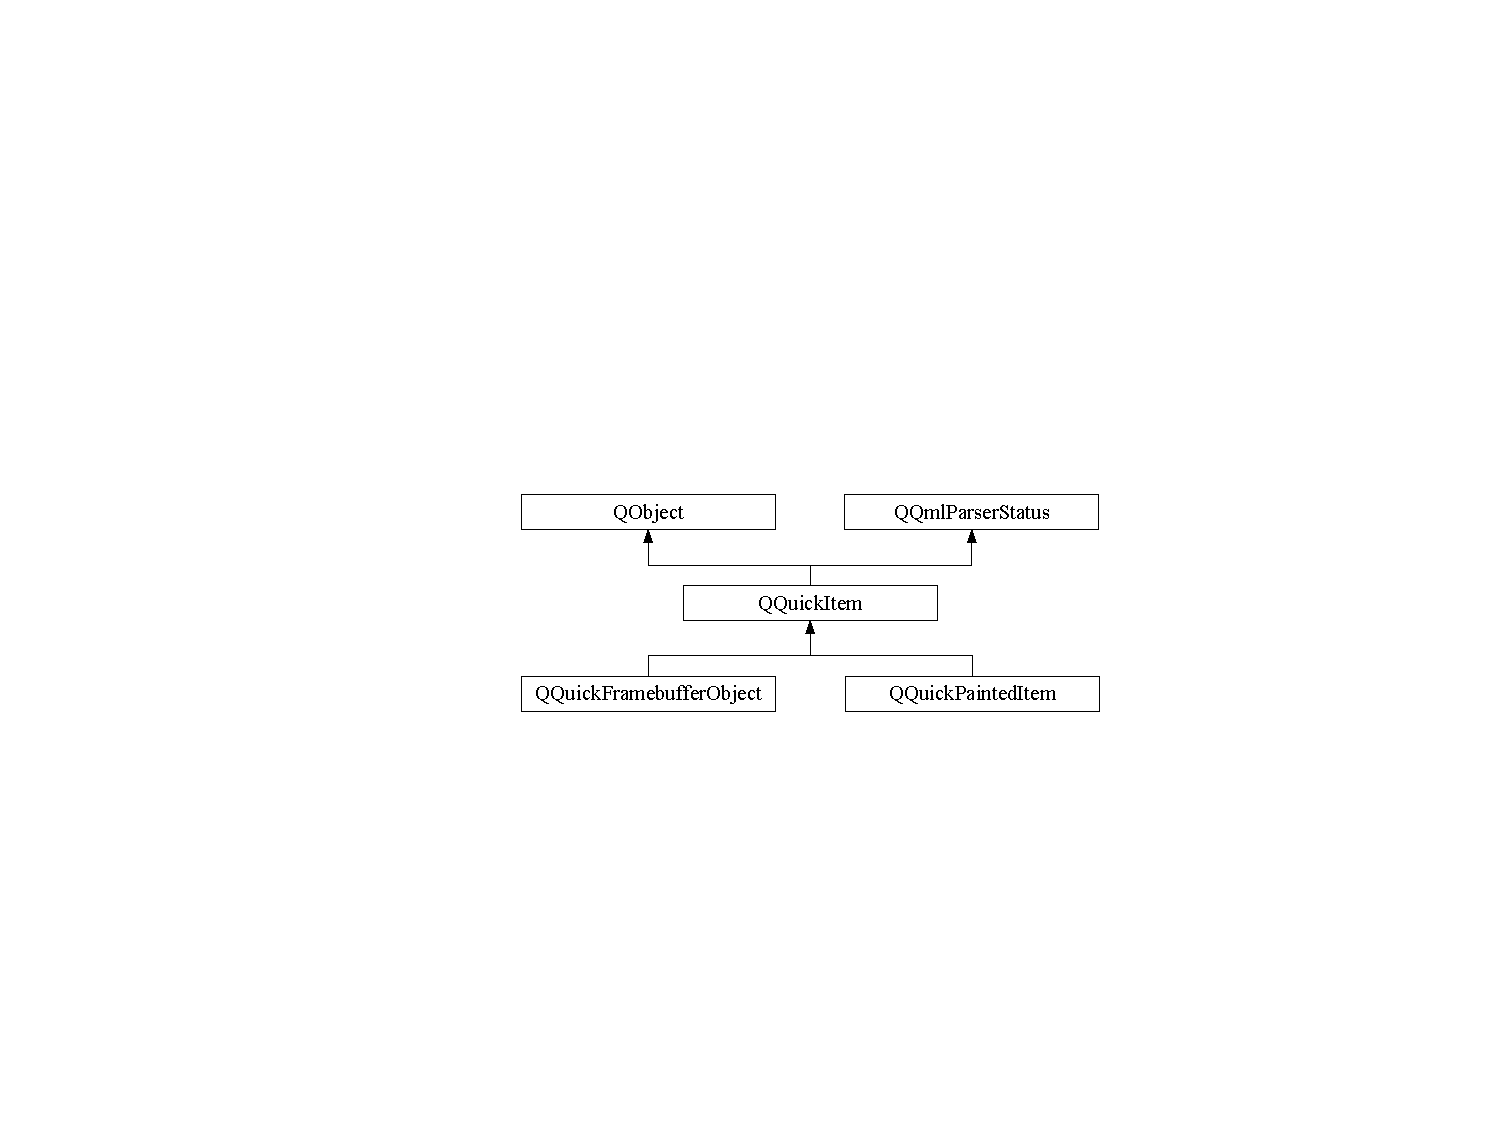
\includegraphics[width=0.95\textwidth]{chapter01/images/qtquick_item.pdf} %图片路径
\caption{C{\sourcefonttwo{}+}{\sourcefonttwo{}+}导出Qt Quick所需基类} %标题
\label{p000010} %索引
\end{figure}
%end图片


本节展示直接使用C{\sourcefonttwo{}+}{\sourcefonttwo{}+}调用OpenGL绘制,并将其导出到Qt Quick。

本节示例位于目录“QtQmlBook/chapter01/directdrawbyopengl”。

%begin图片
\begin{figure}[htb] %浮动体 here and top ...
%there must use marginnote ...
\marginnote{\setlength\fboxsep{2pt}\fbox{\footnotesize{\kaishu\figurename\,}\footnotesize{\ref{p000011}}}}\centering %中心对齐
\setlength\fboxsep{0pt}\fcolorbox[rgb]{0,0,0}{0.97,0.98,0.99}{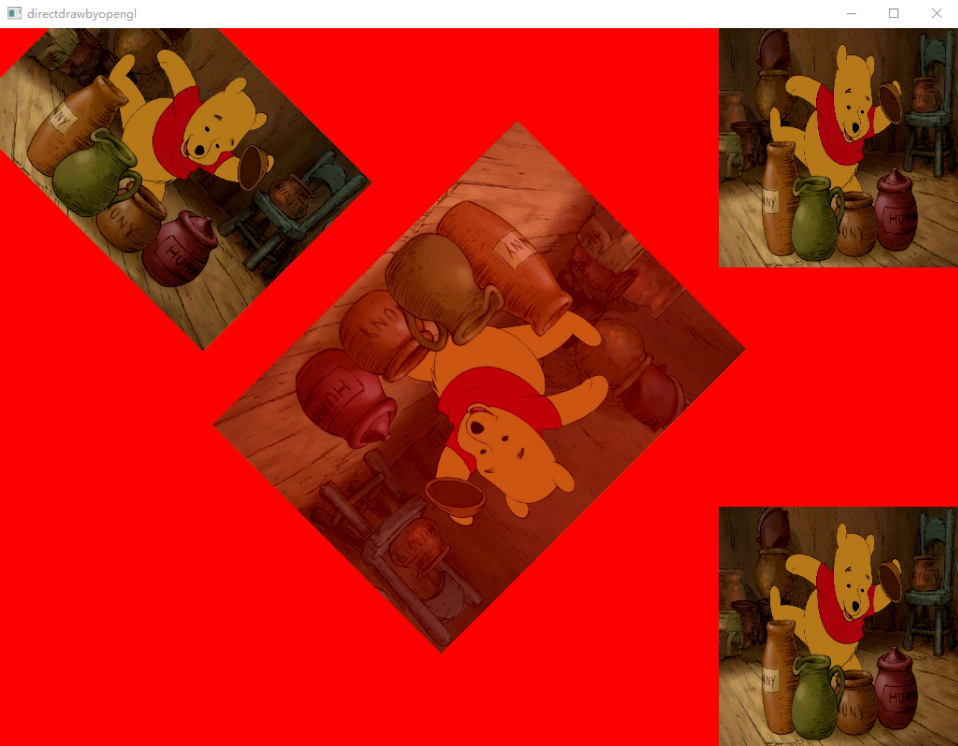
\includegraphics[width=0.95\textwidth]{the_book_image/p000011.pdf}} %图片路径
\caption{直接使用OpenGL绘制} %标题
\label{p000011} %索引
\end{figure}
%end图片


先来看看Qt Quick代码,
如\filesourcenumbernameone\ \ref{f000042}。

%\begin{spacing}{1.0}
\refstepcounter{filesourcenumber}\label{f000042}    %增加源代码编号
\FloatBarrier                                  %强制完成浮动体布局
\begin{thebookfilesourceone}[escapeinside={(*@}{@*)},
caption=GoodLuck,
title=\filesourcenumbernameone \thefilesourcenumber
]
/*directdrawbyopengl/main.qml*/
import QtQuick 2.9
import sstd.quick 1.0

Rectangle{
    id : root_object
    objectName: "root_object";
    width: 1024 ;
    height: 768 ;
    color: Qt.rgba(1,0,0,1);

    DrawImageItemRaw {

        width: parent.width /2  ;
        height: parent.height /2;
        anchors.centerIn: parent;
        transformOrigin: Item.Center ;
        rawImage : Qt.resolvedUrl( "0000.jpg" );

        Timer{
            repeat: true;
            running: true;
            interval : 500 ;
            triggeredOnStart: true;
            onTriggered: {
                parent.rotation += 15 ;
                if(parent.rotation>360){
                    parent.rotation -= 360 ;
                }
                parent.opacity = Math.random() * 0.3 + 0.7 ;
                parent.scale = Math.random() * 0.3 + 0.7   ;
            }
        }

    }


    Component.onCompleted : {
        Qt.createQmlObject(
"
import QtQuick 2.9
import sstd.quick 1.0

DrawImageItemRaw {
    width: 256   ;
    height: 256  ;
    anchors.top: parent.top                 ;
    anchors.right : parent.right            ;
    rawImage : Qt.resolvedUrl( '0000.jpg' ) ;
}

" , root_object  ) ;
    }

}/*Rectangle*/(*@\marginpar[\hfill\setlength\fboxsep{2pt}\fbox{\footnotesize{\kaishu\parbox{1em}{\setlength{\baselineskip}{2pt}\filesourcenumbernameone}}\footnotesize{\thefilesourcenumber}}]{\setlength\fboxsep{2pt}\fbox{\footnotesize{\kaishu\parbox{1em}{\setlength{\baselineskip}{2pt}\filesourcenumbernameone}}\footnotesize{\thefilesourcenumber}}}@*)\end{thebookfilesourceone}          %抄录环境
\addtocounter{lstlisting}{-1}   %sub lstlisting counter ...
%\end{spacing}


\begin{itemize}

\item 第3行引入自定义模块。
其对应的C{\sourcefonttwo{}+}{\sourcefonttwo{}+}代码如\filesourcenumbernameone\ \ref{f000043}:
%\begin{spacing}{1.0}
\refstepcounter{filesourcenumber}\label{f000043}    %增加源代码编号
\FloatBarrier                                  %强制完成浮动体布局
\begin{thebookfilesourceone}[escapeinside={(*@}{@*)},
caption=GoodLuck,
title=\filesourcenumbernameone \thefilesourcenumber
]
static inline void register_this() {
    qmlRegisterType<DrawImageItem>(
        "sstd.quick",
        1, 0,
        "DrawImageItemRaw");
}
Q_COREAPP_STARTUP_FUNCTION(register_this)(*@\marginpar[\hfill\setlength\fboxsep{2pt}\fbox{\footnotesize{\kaishu\parbox{1em}{\setlength{\baselineskip}{2pt}\filesourcenumbernameone}}\footnotesize{\thefilesourcenumber}}]{\setlength\fboxsep{2pt}\fbox{\footnotesize{\kaishu\parbox{1em}{\setlength{\baselineskip}{2pt}\filesourcenumbernameone}}\footnotesize{\thefilesourcenumber}}}@*)\end{thebookfilesourceone}          %抄录环境
\addtocounter{lstlisting}{-1}   %sub lstlisting counter ...
%\end{spacing}


本节的示例依然是静态加载,
实际上Qt Quick也支持以插件的形式动态加载组件。

\item 第12\raisebox{0.16ex}{\sourcefonttwo\~{}}35行演示了如何使用
自定义模块中的类“DrawImageItemRaw”。

使用C{\sourcefonttwo{}+}{\sourcefonttwo{}+}自定义的类与Qt Quick原生元素没有什么不同。
信号槽、平移、旋转、缩放……

不难发现,
使用Qt Quick可以将一切从极高的抽象层上
迅速的组装起来。

\item 第38\raisebox{0.16ex}{\sourcefonttwo\~{}}53行演示了直接在
Qt Quick里面编译Qt Quick源码并以此创建对象。

正如读者所见,
Qt Quick拥有脚本语言的所有特性,
并可以与Qt C{\sourcefonttwo{}+}{\sourcefonttwo{}+}无缝通信。

\end{itemize}

接下来再看看Qt C{\sourcefonttwo{}+}{\sourcefonttwo{}+}主要逻辑代码,
如\filesourcenumbernameone\ \ref{f000044}所
示。

\begin{itemize}

\item 第29\raisebox{0.16ex}{\sourcefonttwo\~{}}44行展示了如何
在Qt C{\sourcefonttwo{}+}{\sourcefonttwo{}+}端从Qml对象树中找到所需对象,并
在Qt C{\sourcefonttwo{}+}{\sourcefonttwo{}+}端创建对象并添加到Qml对象树中。


\item 第46\raisebox{0.16ex}{\sourcefonttwo\~{}}78行展示了如何
在Qt C{\sourcefonttwo{}+}{\sourcefonttwo{}+}端编译Qml并创建对象。

\end{itemize}

%\begin{spacing}{1.0}
\refstepcounter{filesourcenumber}\label{f000044}    %增加源代码编号
\FloatBarrier                                  %强制完成浮动体布局
\begin{thebookfilesourceone}[escapeinside={(*@}{@*)},
caption=GoodLuck,
title=\filesourcenumbernameone \thefilesourcenumber
]
/*directdrawbyopengl/main.cpp*/
#include <sstd_qt_and_qml_library.hpp>
#include "DrawImageItem.hpp"

int main(int argc, char ** argv) {

    /*初始化程序*/
    auto varApp = sstd_make_unique< sstd::Application >(argc, argv);
    /*初始化Qml/Quick引擎*/
    auto varWindow = sstd_make_unique< sstd::DefaultRoowWindow >();
    {
        /*获得Qml文件绝对路径*/
        auto varFullFileName = sstd::getLocalFileFullPath(
            QStringLiteral("myqml/directdrawbyopengl/main.qml"));

        /*加载Qml文件*/
        varWindow->load(varFullFileName);
        /*检查并报错*/
        if (varWindow->status() != sstd::LoadState::Ready) {
            qWarning() << QStringLiteral("can not load : ")
            << varFullFileName;
            return -1;
        }

    }

    varWindow->show();

    {
        /*运行时由C++端添加对象*/
        auto varRootObject = varWindow->getRootObject();
        assert(varRootObject);
        assert(varRootObject->objectName() == QStringLiteral("root_object"));
        auto varItem = sstd_new<DrawImageItem>();
        varItem->setParent(varRootObject);
        const auto varImage = QImage(sstd::getLocalFileFullFilePath(
            QStringLiteral("myqml/directdrawbyopengl/0000.jpg")));
        varItem->setImage(varImage);
        varItem->setWidth(360);
        varItem->setHeight(256);
        varItem->setTransformOrigin(QQuickItem::Center);
        varItem->setRotation(45);
        varItem->setParentItem(varRootObject);
    }

    {
        /*运行时由C++编译QML对象*/
        const auto varQmlCode = u8R"+++(

import QtQuick 2.9
import sstd.quick 1.0

DrawImageItemRaw {

    width: 256                             ;
    height: 256                            ;
    rawImage : Qt.resolvedUrl( "0000.jpg" );
    anchors.bottom: parent.bottom          ;
    anchors.right : parent.right           ;

}

)+++"sv;

        QQmlComponent varComponent{ varWindow->getEngine() };
        auto varContex = QQmlEngine::contextForObject( varWindow->getRootObject() );
        varComponent.setData(
            QByteArray( varQmlCode.data(),static_cast<int>(varQmlCode.size()) ),
            varContex->baseUrl()
        );
        auto varObject = sstd_runtime_cast<DrawImageItem>(
            varComponent.beginCreate( varContex ) );
        assert(varObject);
        varObject->setParent(varWindow->getRootObject());
        varObject->setParentItem(varWindow->getRootObject());
        varComponent.completeCreate();

    }

    return varApp->exec();

}(*@\marginpar[\hfill\setlength\fboxsep{2pt}\fbox{\footnotesize{\kaishu\parbox{1em}{\setlength{\baselineskip}{2pt}\filesourcenumbernameone}}\footnotesize{\thefilesourcenumber}}]{\setlength\fboxsep{2pt}\fbox{\footnotesize{\kaishu\parbox{1em}{\setlength{\baselineskip}{2pt}\filesourcenumbernameone}}\footnotesize{\thefilesourcenumber}}}@*)\end{thebookfilesourceone}          %抄录环境
\addtocounter{lstlisting}{-1}   %sub lstlisting counter ...
%\end{spacing}



% ______all_key_words
% the_book_chapter the_book_subsection the_book_subsubsection
% the_book_section the_book_image the_book_table
% the_book_file the_book_tree_file the_book_command_file
% littlelongworld tabbing ref
% figurename tablename filesourcenumbernameone
% treeindexnumbernameone commandnumbernameone footnote
% item itemize comment textbullet
% \hspace*{\parindent}
% FloatBarrier







%使用XeLaTeX编译
%版权所有,翻版必究
%本文件由程序自动生成,任何修改将被覆盖
%2019 年 01 月 23 日



